% !TEX root = replicas_draft.tex

Hawking famously noted that the process of black hole formation and evaporation seems to create entropy \cite{Hawking:1976ra}. We can form a black hole from a pure state. The formation of the black hole horizon leaves an inaccessible region behind, and the entanglement of quantum fields across the horizon is responsible for the thermal nature of the Hawking radiation as well as its growing entropy. 

A useful diagnostic for information loss is the fine-grained (von Neumann) entropy of the Hawking radiation, $S_R = -\tr \rho_R \log \rho_R$, where $\rho_R$ is the density matrix of the radiation. This entropy initially increases, because the Hawking radiation is entangled with its partners in the black hole interior. But if the evaporation is unitary, then it must eventually fall back to zero following the Page curve \cite{Page:1993wv,Page:2013dx}.  On the other hand, Hawking's calculation predicts an entropy that rises monotonically as the black hole evaporates. 


Hawking's computation of the entropy seems straightforward. It can be done far from the black hole where the
effects of quantum gravity are small, so it is unclear what could have gone wrong. 
An answer to this puzzle was recently proposed \cite{Penington:2019npb,Almheiri:2019psf,Almheiri:2019hni}  (see also 
\cite{Mertens:2019bvy,Akers:2019wxj,Moitra:2019xoj,Almheiri:2019psy,Fu:2019oyc,Zhang:2019fcy,Akers:2019nfi,Almheiri:2019yqk,Rozali:2019day,Chen:2019uhq,Bousso:2019ykv,Jafferis:2019wkd,Blommaert:2019wfy}). The proposal is that Hawking used the wrong formula for computing the entropy. As the theory is coupled to gravity, we should use the proper gravitational formula for entropy: the gravitational fine-grained entropy formula studied by Ryu and Takayanagi \cite{Ryu:2006bv} and extended in \cite{Hubeny:2007xt,Faulkner:2013ana,Engelhardt:2014gca}, also allowing for 
spatially disconnected regions, called ``islands,'' see 
 figure \ref{fig:QESreview}.  Even though the radiation lives in a region where the gravitational effects are small, the fact that we are describing a state in a theory of gravity 
 implies that we should use the gravitational formula for the entropy, including the island rule. 
 


\begin{figure}
\begin{center}
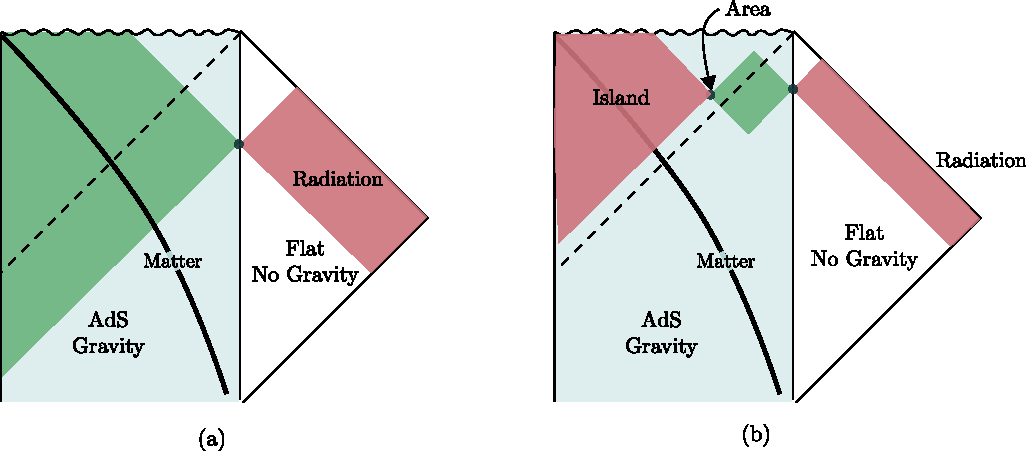
\includegraphics[scale=0.8]{figures/evaporation-island.pdf}
\end{center}
\caption{  We display an evaporating black hole. The vertical line separates a region on the left where gravity is dynamical from a region on the right where we can approximate it as not being dynamical. The black hole is evaporating into this second region. In red we see the regions associated to the computation of the entropy of radiation and in green the regions computing the entropy of the black hole. (a) Early times. (b) Late times, where we have an island. } 
\label{fig:QESreview}
\end{figure}


In this paper we consider a version of the information paradox formulated recently in \cite{Penington:2019npb,Almheiri:2019psf} (see also \cite{Mathur:2014dia})
where a black hole in anti-de Sitter spacetime radiates into an attached Minkowski region.  We show that the first principles computation of the fine-grained entropy using the gravitational path integral description   receives large corrections from non-perturbative effects. The effects come from new saddles in the gravitational path integral --- replica wormholes --- that dominate over the standard Euclidean black hole saddle, and lead to a fine-grained entropy consistent with unitarity.   



We will discuss the saddles explicitly only in some simple examples related to the information paradox for eternal black holes in two-dimensional Jackiw-Teitelboim (JT) gravity \cite{Jackiw:1984je,Teitelboim:1983ux,Almheiri:2014cka}, reviewed below, but we can nonetheless compute the effect on the fine-grained entropy more generally.
The same answer for the entropy was obtained holographically in \cite{Almheiri:2019hni,Chen:2019uhq,Rozali:2019day}. 
Our goal is to provide a direct, bulk derivation   without using holography.




To summarize our approach briefly, we will revisit the calculation of the von Neumann entropy of radiation outside a black hole in AdS glued to flat space, using the replica method. We introduce $n$ copies of the original black hole, analytically continue to non-integer $n$, and compute the von Neumann entropy as $S_R = - \p_n \tr (\rho_R)^n|_{n = 1}$. Since the theory is coupled to gravity, we must do the gravitational path integral  to calculate $\tr (\rho_R)^n$. Under our assumptions about the matter content, this path integral is dominated by a saddlepoint. There is one obvious saddle, in which the geometry is $n$ copies of the original black hole; this saddle leads to the standard Hawking result for the von Neumann entropy, \textit{i.e.}, the entropy of quantum fields in a fixed curved spacetime, see figure \ref{fig:2wormhole}(a).

 

 
 There is, however, another class of saddles in which the different replicas are connected by a new geometry. These are the replica wormholes, see figure \ref{fig:2wormhole}(b), \ref{fig:manyreplicas}. In the examples we consider, whenever the Hawking-like calculation leads to an entropy in tension with unitarity, the replica wormholes start to dominate the gravitational path integral, and resolve the tension.

 
Our use of the replica trick in a theory coupled to gravity closely parallels the derivation of   the Ryu-Takayanagi formula  and its generalizations \cite{Lewkowycz:2013nqa,Faulkner:2013ana,Dong:2016hjy,Dong:2017xht}.

In the rest of the introduction we summarize the main idea in more detail.

Similar ideas are explored independently in a paper by Penington, Shenker, Stanford, and Yang \cite{Penington:2019kki}.

\subsection{The island rule for computing gravitational von Neumann entropies}

We begin by reviewing the recent progress on the information paradox in AdS/CFT  \cite{Penington:2019npb,Almheiri:2019psf}.

The classic information paradox is difficult to study in AdS/CFT, because large black holes do not evaporate. Radiation bounces off the AdS boundary and falls back into the black hole.  For this reason, until recently, most discussions of the information paradox in AdS/CFT have focused on exponentially small effects, such as the late-time behavior of boundary correlation functions \cite{Maldacena:2001kr,Saad:2018bqo,Saad:2019lba,Saad:2019pqd}.

In contrast, the discrepancy in the Page curve is a large, $O(1/G_N)$, effect. This classic version of the information paradox can be embedded into AdS/CFT by coupling AdS to an auxiliary system that absorbs the radiation, allowing the black hole to evaporate \cite{Penington:2019npb,Almheiri:2019psf} (see also \cite{Rocha:2008fe, Mertens:2019bvy, Engelsoy:2016xyb}). This is illustrated in fig.~\ref{fig:QESreview} in the case where the auxiliary system is half of Minkowski space, glued to the boundary of AdS. There is no gravity in the Minkowski region, where effectively $G_N \to 0$, but radiation into matter fields is allowed to pass through the interface.

In this setup, the Page curve of the black hole was calculated   in 
\cite{Penington:2019npb,Almheiri:2019psf}. It is important to note that this calculation gives the Page curve of the black hole, not the radiation, which is where the paradox lies; we return to this momentarily.
The entropy of the black hole is given by the generalized entropy of the quantum extremal surface (QES) \cite{Engelhardt:2014gca}, which is a quantum-corrected  Ryu-Takayanagi (or Hubeny-Rangamani-Takayanagi) surface \cite{Ryu:2006bv,Hubeny:2007xt}. According to the QES proposal, the von Neumann entropy of the black hole is
\be\label{introsbh}
S_B = \mbox{ext}_Q \left[ \frac{\mbox{Area}(Q)}{4G_N} + S_{\rm matter}(B) \right]
\ee
where $Q$ is the quantum extremal surface, and $B$ is the region between $Q$ and the AdS boundary. $S_{\rm matter}$ denotes the von Neumann entropy of the  quantum field theory (including perturbative gravitons) calculated in the fixed background geometry. The extremization is over the choice of surface $Q$. If there is more than one extremum, then $Q$ is the surface with minimal entropy. For dilaton gravity in AdS$_2$, $Q$ is a point, and its `area' means the value of the dilaton.





The black hole Page curve  is the function $S_B(t)$, where $t$ is the time on the AdS boundary where $B$ is anchored. 
It depends on time  because the radiation can cross into the auxiliary system. 
It behaves as expected: it grows at early times, then eventually falls back to zero \cite{Penington:2019npb,Almheiri:2019psf}. A crucial element of this analysis is that at late times, the dominant quantum extremal surface sits near the black hole horizon, as in fig.~\ref{fig:QESreview}.

This does not resolve the Hawking paradox, 
 which involves the radiation entropy $S_{\rm matter}(R)$, where $R$ is a region outside the black hole containing the radiation that has come out. 
Clearly the problem is that neither $R$ nor $B$ includes the region $I$ behind the horizon, called the island, 
see figure \ref{fig:QESreview}. The state of the quantum fields on $R \cup B$ is apparently not pure, and, apparently  $S_R \neq S_B$. Only if we assume unitarity, or related holographic input such as entanglement wedge reconstruction \cite{Penington:2019npb}, can we claim that the QES computes the entropy of the radiation.  
It does, however, tell us what to aim for in a unitary theory.

 With this motivation, in \cite{Almheiri:2019hni}, the evaporating black hole in Jackiw-Teitelboim (JT) gravity in AdS$_2$ was embedded into a holographic theory in one higher dimension. The AdS$_2$ black hole lives on a brane at the boundary of AdS$_3$, similar to a Randall-Sundrum model \cite{Randall:1999vf,Karch:2000ct}, with JT gravity on the brane (see also \cite{Almheiri:2019psy} for an analogous construction on an AdS$_4$ boundary of AdS$_5$). In this setup, \cite{Almheiri:2019hni} derived the QES prescription \textit{for the radiation} using AdS$_3$ holography. It was found that the von Neumann entropy of the radiation in region $R$, computed holographically in AdS$_3$, agrees with the black hole entropy in \eqref{introsbh}. This led to the conjecture that in a system coupled to gravity, the ordinary calculation of von Neumann entropy should be supplemented by the contribution from ``islands" according to the following rule:
\be \la{IslRule}
S(\rho_R) = \mbox{ext}_Q \left[ \frac{\mbox{Area}(Q)}{4G_N} + S(\tilde{\rho}_{I \cup R}) \right] \ ,
\ee
up to subleading corrections. Here $\rho_R$ is the density matrix of the region $R$ in the full theory coupled to quantum gravity, and $\tilde{\rho}_{I \cup R}$ is the density matrix of the state prepared via the semi-classical path integral on the Euclidean black hole saddle.
This is equal to \eqref{introsbh}, since the quantum fields are pure on the full Cauchy slice $I \cup B \cup R$. Thus the tension with unitarity is resolved within three-dimensional holography.

In this paper we explain how the surprising island rule \nref{IslRule} follows from the standard rules for computing gravitational fine-grained entropy,   without appealing to   higher dimensional holography. 



\subsection{Two dimensional eternal black holes and the information paradox}

We consider an AdS$_2$   JT gravity theory coupled to a 2d CFT. This CFT also lives in   non-gravitational Minkowski regions, and has transparent boundary conditions at the $AdS$ boundary. 
 The dilaton goes to infinity at the AdS$_2$ boundary so it is consistent to freeze gravity on the outside \cite{Engelsoy:2016xyb,Almheiri:2019psf}. We will assume that the matter CFT has a large central charge $c \gg 1$, but we will not assume that it is holographic, as all our calculations are done directly in the 2d theory. For example it could be $c$ free bosons. Taking the central charge large is to suppress the quantum fluctuations of the (boundary) graviton relative to the matter sector. 

This simple model of an $AdS_2$ black hole glued to flat space can be directly applied to certain four dimensional 
 black holes. For example, for the near extremal magnetically charged black holes discussed in \cite{Maldacena:2018gjk}, at low temperatures we can approximate the dynamics as an $AdS_2$ region joined to a flat space region, and the light fields come from effectively two dimensional fields moving in the radial and time direction that connect the two regions. 

We will consider a simple initial state which is the thermofield double state for the black hole plus radiation. 
This state is prepared by a simple Euclidean path integral, see figure \ref{fig:TFDpreparation}. The resulting
Lorentzian geometry is shown in figure \ref{fig:eternalBH-lorentzian}. 


\begin{figure}
\begin{center}
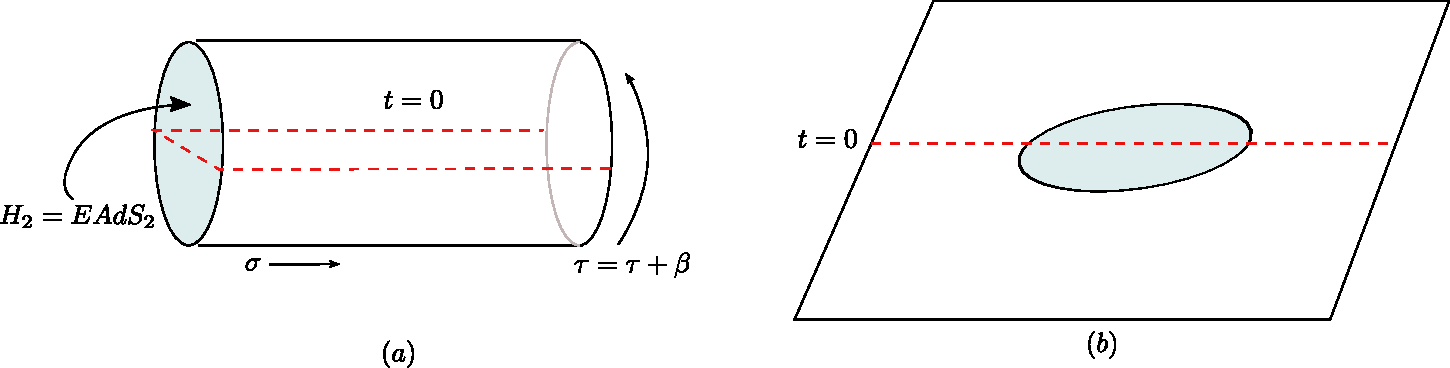
\includegraphics[scale=0.6]{figures/thermal-state.pdf}
\end{center}
\caption{We prepare the combined thermofield double state of the black hole and radiation using a Euclidean path integral. These are two pictures for the combined geometry. In   (b) we have represented the outside cylinder as the outside of the disk. By cutting along the red dotted line, we get our desired thermofield double initial state that we can then use for subsequent Lorentzian evolution (forwards or backwards in time) to get 
the diagram in figure \ref{fig:eternalBH-lorentzian}.  } 
\label{fig:TFDpreparation}
\end{figure}


\begin{figure}
\begin{center}
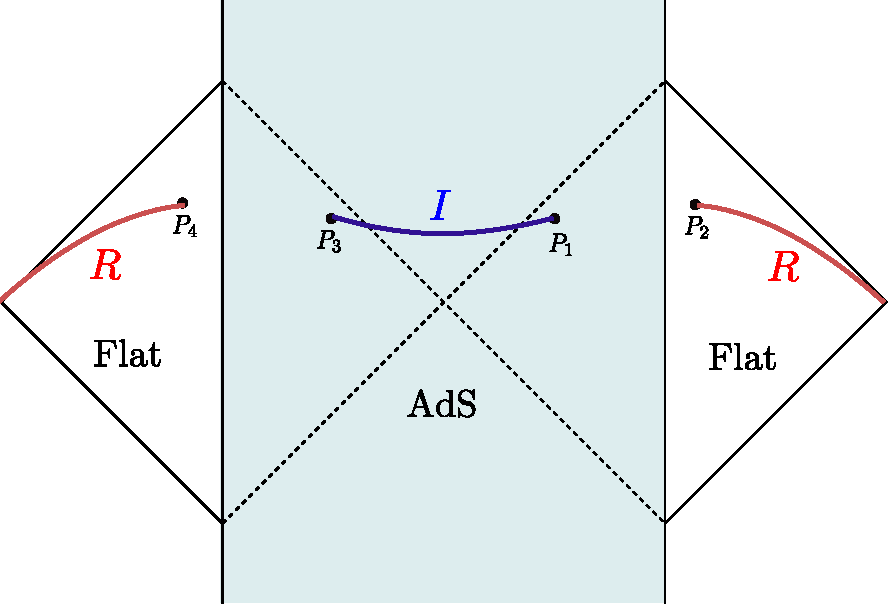
\includegraphics[scale=0.6]{figures/eternalBH-lorentzian.pdf}
\end{center}
\caption{Eternal black hole in AdS$_2$, glued to Minkowski space on both sides. Hawking radiation is collected in region $R$, which has two disjoint components. Region $I$ is the island. The shaded region is coupled to JT gravity. 
} 
\label{fig:eternalBH-lorentzian}
\end{figure}

Despite its simplicity, this setup exhibits Hawking's information paradox, and the corresponding puzzle with the Page curve \cite{Page:1993wv,Page:2013dx}. To reach a paradox, we collect Hawking radiation in region $R$ in figure
\ref{fig:eternalBH-lorentzian}. As a function of time, $R$ moves upward on both sides of the Penrose diagram, so this is not a symmetry. Indeed, the von Neumann entropy of the radiation as calculated by Hawking, $S_{\rm matter}(R(t))$, grows linearly with time, see fig.~\ref{Page}. 
 The origin of this growth is the following. At $t=0$ the radiation modes on the left are entangled with modes on the right. However, as time progresses some of these modes fall into the black holes, others are replaced by black hole modes, see figure 
\ref{fig:Cartoon}. 

If this growth were to continue forever,  it would become larger  than the 
 Bekenstein-Hawking entropies of the two black holes, and this is a contradiction.  See a related discussion 
 of the critically illuminated black hole in flat spacetime in \cite{Fiola:1994ir}. 
 
In a unitary theory, $S_R(t)$ should saturate at around the twice the  Bekenstein-Hawking entropy of each black hole, see figure \ref{Page}. This was confirmed using the island rule in \cite{Almheiri:2019yqk}.

 

\begin{figure}
\begin{center}
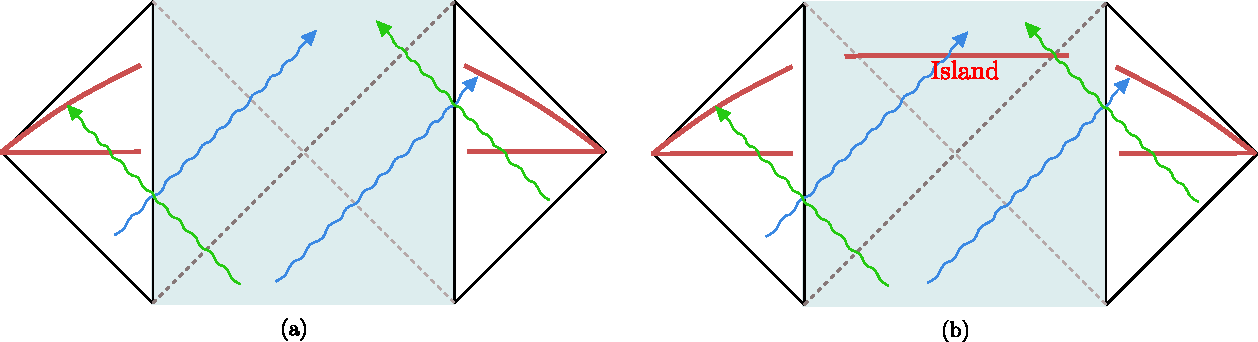
\includegraphics[scale=0.7]{figures/island-pairs.pdf}
\end{center}
\caption{(a) Growing entropy for the radiation for an eternal black hole plus radiation in the thermofield double state. We draw two instants in time. The particles with the same color are entangled. They do not contribute to the entanglement of the radiation region (indicated in red) at $t=0$ but they do contribute at  a later value of $t$. (b) When the island is included the entanglement ceases to grow, because now   both entangled modes mentioned above are included in $I \cup R$.    } 
\label{fig:Cartoon}
\end{figure}

\begin{figure}
\begin{center}
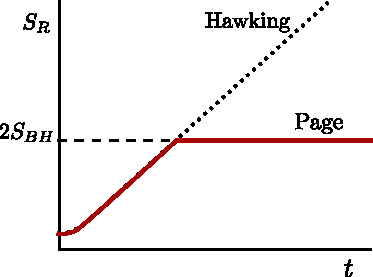
\includegraphics[scale=1]{figures/eternal-page-curve.pdf}
\end{center}
\caption{  Page curve for the entropy of the radiation, for the model in fig. \ref{fig:eternalBH-lorentzian}. The dotted line is the growing result given by the Hawking computation, and the entropy calculated from the other saddle is dashed. The minimum of the two is the Page curve for this model.     } 
\label{Page}
\end{figure}


\subsection{Replica wormholes to the rescue}

To reproduce the unitary answer directly from a gravity calculation, we will use the replica method to compute the von Neumann entropy of region $R$. The saddles relevant to the unitary Page curve will ultimately be complex solutions of the gravitational equations. The idea is to do Euclidean computations and then analytically continue to Lorentzian signature. 


\begin{figure} 
\begin{center}

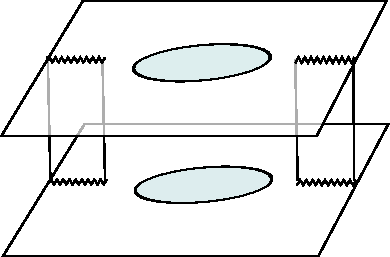
\includegraphics[scale=.9]{figures/replica2-hawking.pdf} \hspace{20mm}
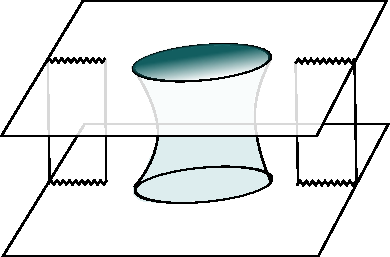
\includegraphics[scale=.9]{figures/replica2-wormhole.pdf}  

 (a) ~~~~~~~~~~~~~~~~~~~~~~~~~~~~~~~~~~~~~~~~~~~~~~~~~~~~~~~~~~~~~~(b)
	\end{center}
\caption{\small Two different saddlepoint contributions to the two-replica path integral in the presence of gravity in the shaded region. On the left the replicas are sewn together along the branch points, outside of the shaded region, as we would do in an ordinary quantum field theory calculation. These will give the standard QFT answer, as computed by Hawking, which can lead to a paradox. On the right we have a saddle where gravity dynamically glues together the shaded regions. This is the replica wormhole. In the examples considered in this paper, this saddle dominates in the relevant kinematics, leading to a Page curve consistent with unitarity. \label{fig:2wormhole}}
\end{figure}

Consider $n=2$ replicas. The replica partition function $\tr (\rho_R)^2$ is computed by a Euclidean path integral on two copies of the Euclidean system, with the matter sector sewed together along the cuts on region $R$. Since we are doing a gravitational path integral, we do not specify the geometry in the gravity region; we only fix the boundary conditions at the edge. Gravity then fills in the geometry  dynamically, see fig.~\ref{fig:2wormhole}. 

We consider two different saddles with the correct boundary conditions.  The first is the Hawking saddle, see
figure  \ref{fig:2wormhole}(a). The corresponding von Neumann entropy is the usual answer, $S_{\rm matter}(R(t))$, which grows linearly forever. The second is the replica wormhole, which, as we will show,  reproduces the entropy of the island rule, see figure  \ref{fig:2wormhole}(b). A replica wormhole with higher $n$ is illustrated in fig.~\ref{fig:manyreplicas}.


\begin{figure}
\begin{center}
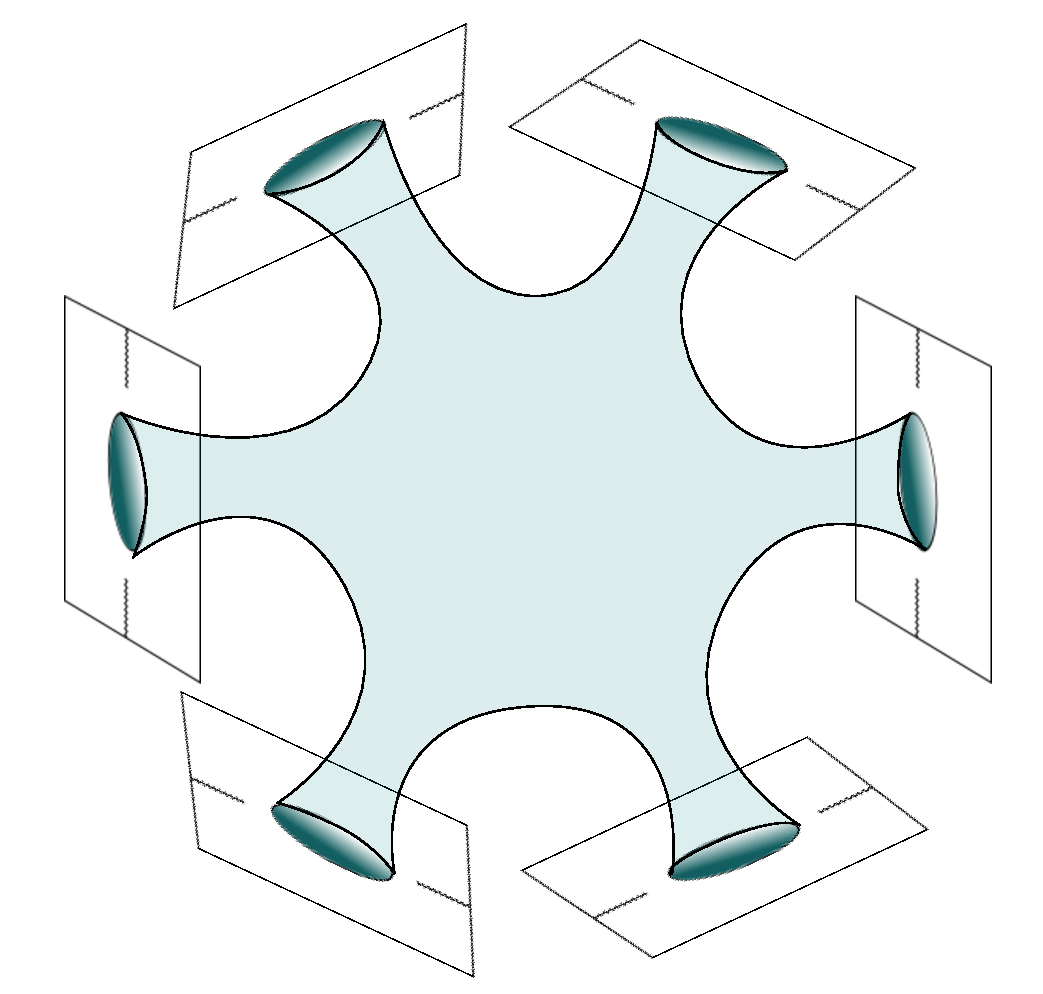
\includegraphics[scale=0.4]{figures/manyreplicas.pdf}
\end{center}
\caption{\small Topology of a replica wormhole with $n=6$. The sheets are also glued together cyclically along the cuts in the matter region. \label{fig:manyreplicas}}
\end{figure}



Replica wormholes have higher topology, so they are suppressed by factors of $e^{-S_0}$ where $S_0$ is the genus-counting parameter of JT gravity. At late times, the contribution of the Hawking saddle is heavily suppressed by the kinematics, and this is what makes it possible for the replica wormhole to take over despite the topological suppression. Indeed, the
$n^{th}$ wormhole, see fig. \ref{fig:manyreplicas}, gives a partition function $Z_n \propto 
e^{ S_0 (2 -n) } $ which leads to a $2S_0$ contribution to the  entropy.  

The wormhole topology has a saddle point at finite $n$. (We will not show this in general, but confirm it explicitly in certain limits; see below for details.) The equations that control this saddle point can be analytically continued to non-integer $n$, and used to define the replica limit $n \to 1$. 
To analyze this limit it is most convenient to assume replica symmetry and go to a quotient space which has a simpler topology but contains conical singularities and insertions of twist operators for the matter 
fields, see figure \ref{CoverThree}. In the limit $n\to 1$ both of these effects become very small and represent a small perturbation for the geometry, but they give a contribution to the entropy of precisely the same form as the gravitational generalized entropy for regions in the $n=1$ solution. The boundaries of the regions are specified by the locations of the twist operators. The replica wormholes give rise to the island contributions to the   entropy.


The physical picture that descends from accounting for these higher
topology saddles in the entropy calculation is as follows. In the
initial stages of the black hole evaporation, the quantum state of the
Hawking radiation is accurately described by quantum field theory on a
fixed background as originally studied by Hawking. This is accurate up to the Page time, defined to be the time when 
the semi-classical von Neumann
entropy of the Hawking radiation becomes equal to the the coarse-grained entropy
of the black hole. 
 At later times,  a non-perturbative effect in the gravitational path
integral results in an $O(1)$ deviation of the evolution of the
entropy of the Hawking radiation form the semi-classical result. This
is due to an exchange of dominance between the trivial topology
saddle and the wormhole saddle in the Renyi entropy calculation. This
new saddle suggests that we should think of the inside of the black hole as
a subsystem of the outgoing Hawking radiation. Namely, in the $n\to 1$ limit of the the replica trick, most of the black hole interior is included, together with the radiation, in the computation of the entropy.  This has the effect
that entanglement across the event horizon of the Hawking pairs no
longer contributes to the von Neumann entropy of the outgoing part,
while at the same time maintaining the necessary entanglement to
ensure semi-classical physics at the horizon.
  
 This paper is organized as follows. 

In section \ref{sec:CosmicStrings} we review and slightly clarify the gravitational derivation of the quantum extremal surface presciption from the replica trick in a general theory \cite{Lewkowycz:2013nqa,Faulkner:2013ana,Dong:2016hjy,Dong:2017xht}. The slight improvement is that we show that the off shell action near $n\sim 1$ becomes the generalized entropy, so that the extremality condition follows directly from the 
extremization of the action. In section 
\ref{JTplusCFT} we discuss some general aspects of replica manifolds for the case of JT gravity plus a CFT. 

In section \ref{sec:SingleInterval} we discuss the computation of the entropy for an interval that contains the degrees of freedom living at the $AdS$ boundary. In this case the quantum extremal surface is slightly outside the horizon. We set up the discussion of the Renyi entropy computations for this case. We reduce the problem to an integro-differential equation for a single function $\theta(\tau)$ that relates the physical time $\tau$ to the $AdS$ time $\theta$. We solve this equation for $n\to 1$ recovering the quantum extremal surface result. We also solve the problem for relatively high temperatures but for any $n$. 

In section \ref{sec:OneZero} we discuss the special case of the zero temperature limit, and we comment on some features of the island in that case. 

In section \ref{sec:TwoIntervals} we discuss aspects of the two intervals case, which is the one most relevant for the information problem for the eternal black hole.  

In section \ref{sec:Dictionary} we make the connection to entanglement wedge reconstruction of the black hole interior.

 We end in section \ref{sec:Conclusions} with conclusions and discussion. 
 

